% Tame Graphs
% Thomas C. Hales
% Starting with Chapter on Tame Plane Graphs


\label{sec:tame}


\chapter{Tame Graphs}
\label{sec:def-and-class}

This \chap\ defines a class of plane graphs.  Graphs in this class
are said to be {\it tame}.  In the next \chap, we give a complete
classification of all tame graphs.  This classification of tame
graphs was carried out by computer. This classification is a major
step of the proof of the Kepler conjecture.

\section{Basic Definitions}

\begin{definition}
An {\it n-cycle\/} is a finite set $C$ of cardinality $n$,
together with a cyclic permutation $s$ of $C$.   We write $s$ in
the form $v\mapsto s(v,C)$, for $v\in C$.  The element $s(v,C)$ is
called the {\it successor\/} of $v$ (in $C$).  A {\it cycle\/} is
a $n$-cycle for some natural number $n$. By abuse of language, we
often identify $C$ with the cycle. The natural number $n$ is the
{\it length\/} of the cycle.
%
 \index{cycle}
 \index{successor}
 \index{sZ@$s(v,C)$}
 \index{length (of a cycle)}
 \index{cycle!length}
\end{definition}

%(We may assume that all vertices of all graphs lie in some large
%finite set of vertices $\Omega$, if we wish to arrange that only
%finitely many graphs occur in this discussion.)

\begin{definition}
Let $G$ be a nonempty finite set of cycles (called faces) of
length at least $3$. The elements of faces are called the {\it
vertices} of $G$. An unordered pair of vertices $\{v,w\}$ such
that one element is the successor of the other in some face is
called an {\it edge}. The vertices $v$ and $w$ are then said to be
{\it adjacent}. The set $G$ is a {\it plane graph} if four
conditions hold.
%
 \index{plane graph}
 \index{vertex}
 \index{adjacent}
 \index{face}
 \index{edge (of a plane graph)}
    \begin{enumerate}
    \item If an element $v$ has successor $w$ in some face $F$, then
there is a unique face (call it $s'(F,v)$) in $G$ for which $v$ is
the successor of $w$. (Thus, $v=s(w,s'(F,v))$, and each edge
occurs twice with opposite orientation.)
    \item  For each vertex $v$, the function $F\mapsto s'(F,v)$ is
    a cyclic permutation of the set of faces containing $v$.
    \item  Euler's formula holds relating the number of vertices $V$, the
number of edges $E$, and the number of faces $F$:
    $$V-E+F = 2.$$
    \item The set of vertices is connected.  That is, the only nonempty
    set of vertices that is closed under $v\mapsto s(v,C)$ for all $C$
    is the full set of vertices.
    \end{enumerate}
\end{definition}

\begin{remark} The set of vertices and edges of a plane graph form a planar
graph in the usual graph-theoretic sense of admitting an embedding
into the plane.  Every planar graph carries an orientation on its
faces that is inherited from an orientation of the plane. (Use the
right-hand rule on the face, to orient it with the given outward
normal of the oriented plane.)  For us, the orientation is built
into the definition, so that properly speaking, we should call
these objects {\it oriented plane graphs}.  We follow the
convention of distinguishing between planar graphs (which admit an
embedding into the plane) and plane graphs (for which a choice of
embedding has been made).  Our definition is more restrictive than
the standard definition of plane graph in the literature, because
we require all faces to be simple polygons with at least $3$
vertices.  Thus, a graph with a single edge does not comply with
our narrow definition of plane graph. Other graphs that are
excluded by this definition are shown in
Figure~\ref{fig:nonplanar}.  Standard results about plane graphs
can be found in any of a number of graph theory textbooks.
However, this paper is written in such a way that it should not be
necessary to consult outside graph theory references.
 %
 \index{plane graph}
 \index{planar graph}
\end{remark}

    \begin{figure}[htb]
        \centering
        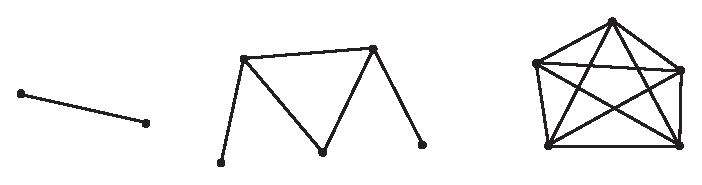
\includegraphics{PS/nonplanar.eps}
        \caption{Some examples of graphs that are excluded from the
        narrow definition of plane graph, as defined in this section.}
        \label{fig:nonplanar}
    \end{figure}

\begin{definition}
Let $len$ be the length function on faces.  Faces of length $3$
are called {\it triangles}, those of length $4$ are called {\it
quadrilaterals}, and so forth. Let $tri(v)$ be the number of
triangles containing a vertex $v$. A face of length at least $5$
is called an {\it exceptional\/} face.
 %
 \index{triangle}
 \index{exceptional}
 \index{quadrilateral}
 \index{exceptional!face}
 \index{tZri@$tri(v)$}
\end{definition}

Two plane graphs are {\it properly} isomorphic if there is a
bijection of vertices inducing a bijection of faces.  For each
plane graph, there is an opposite plane graph $G^{op}$ obtained by
reversing the cyclic order of vertices in each face.  A plane
graph $G$ is  isomorphic to another if $G$ or $G^{op}$ is properly
isomorphic to the other.
%
 \index{proper isomorphism}

\begin{definition}
The {\it degree\/} of a vertex is the number of faces it belongs
to. An {\it $n$-circuit\/} in $G$ is a cycle $C$ in the vertex-set
of $G$, such that for every $v\in C$, it forms an edge in $G$ with
its successor: that is, $(v,s(v,C))$ is an edge of $G$.
%
 \index{degree (of a vertex)}
 \index{circuit}
\end{definition}

In a plane graph $G$ we have a combinatorial form of the Jordan
curve theorem: each $n$-circuit determines a partition of $G$ into
two sets of faces.

\begin{definition}\label{definition:type}
The {\it type\/} of a vertex is defined to be a triple of
nonnegative integers $(p,q,r)$, where $p$ is the number of triangles
containing the vertex, $q$ is the number of quadrilaterals
containing it, and $r$ is the number of exceptional faces. When
$r=0$, we abbreviate the type to the ordered pair $(p,q)$.
%
 \index{type (of a vertex)}
\end{definition}


\section{Weight Assignments}\label{sec:wtassign}

We call the constant $\op{tgt}=14.8$, which arises repeatedly in
this section, the {\it target}.  (This constant arises as an
approximation to $4\pi\zeta -8\approx 14.7947$, where $\zeta =
1/(2\arctan(\sqrt{2}/5))$.)
%
 \index{target}\index{tgt@$\op{tgt}=14.8$}
 \index{ZZdzeta@$\zeta= 1/(2\arctan(\sqrt{2}/5))$}

  Define $a:\N\to \R$ by
  $$a(n) = \begin{cases}
    14.8 &n=0,1,2,\\
    1.4 & n=3,\\
    1.5 & n=4,\\
    0 & \text{otherwise.}
  \end{cases}
  \index{aZ@$a(n)$}
  $$
  Define $b:\N\times \N\to \R$ by $b(p,q)=14.8$,
  except for the values in the following table
  (with  $\op{tgt}=14.8$):
  {
  \def\tx{\op{tgt}}
  $$\begin{matrix}  &q=0&1&2&3&4\\
           p=0&\tx&\tx&\tx&7.135&10.649\\
           1&\tx&\tx&6.95&7.135&\tx\\
           2&\tx&8.5&4.756&12.981&\tx\\
           3&\tx&3.642&8.334&\tx&\tx\\
           4&4.139&3.781&\tx&\tx&\tx\\
           5&0.55&11.22&\tx&\tx&\tx\\
           6&6.339&\tx&\tx&\tx&\tx
   \end{matrix}
   \index{bZ@$b(p,q)$}
   $$
   }
  Define $c:\N\to \R$ by
  $$c(n) = \begin{cases}
    1 & n=3,\\
    0 & n=4,\\
    -1.03 &n=5,\\
    -2.06 &n=6,\\
    -3.03 &\text{otherwise.}
    \end{cases}
    \index{cZ@$c(n)$}
    $$
    Define $d:\N\to \R$ by
  $$d(n) = \begin{cases}
    0 & n=3, \\
    2.378 & n=4, \\
    4.896 & n=5, \\
    7.414 & n=6, \\
    9.932 & n=7, \\
    10.916 & n=8,\\
    \op{tgt}=14.8 & \text{otherwise}.
  \end{cases}
  \index{dZ@$d(n)$}
  $$

A set $V$ of vertices is called a {\it separated\/} set of
vertices if the following four conditions hold.
%
 \index{separated set}
    \begin{enumerate}
      \item For every vertex in $V$ there is an exceptional face
         containing it.
      \item No two
        vertices in $V$ are adjacent.
      \item No two vertices
        in $V$ lie on a common quadrilateral.
      \item Each vertex in $V$ has degree 5.
    \end{enumerate}

%
A {\it weight assignment\/} of a plane graph $G$ is a function
$w:G\to \R$ taking values in the set of nonnegative real numbers. A
weight assignment is {\it admissible} if the following properties
hold:
%
 \index{weight assignment}
 \index{admissible (weight assignment)}
\begin{enumerate}
  \item If the face $F$ has length $n$, then
        $w(F) \ge d(n)$
  \item If $v$ has type $(p,q)$, then
        $$\sum_{F:\,v\in F} w(F) \ge b(p,q).$$
        \label{admissible:b}
  \item Let $V$ be any set of vertices of type $(5,0)$.
        If the cardinality of $V$ is $k\le 4$,
        then
        $$\sum_{F:\,V\cap F\ne\emptyset} w(F) \ge 0.55 k.$$
  \item Let $V$ be any separated set of vertices.
        Then
        $$\sum_{F:\,V\cap F\ne\emptyset} (w(F) -d(len(F)))
            \ge \sum_{v\in V} a(tri(v)).$$
        \label{definition:admissible:excess}
\end{enumerate}

 The sum
$\sum_F w(F)$ is called the {\it total weight} of $w$.
\index{total weight}


\section{Plane Graph Properties}
\label{sec:graphproperty}

We say that a plane graph is {\it tame\/} if it satisfies the
following conditions.
%
 \index{tame}

\begin{enumerate}
    \label{definition:tame}
    \item The length of each face is at least $3$ and at most $8$.
    \label{definition:tame:length}

    \item Every $3$-circuit is a face or the opposite of a face.
    \label{definition:tame:3-circuit}

    \item Every $4$-circuit surrounds one of the cases illustrated in Figure
    \ref{fig:fourcircuit}.
    \label{definition:tame:4-circuit}
    \begin{figure}[htb]
        \centering
        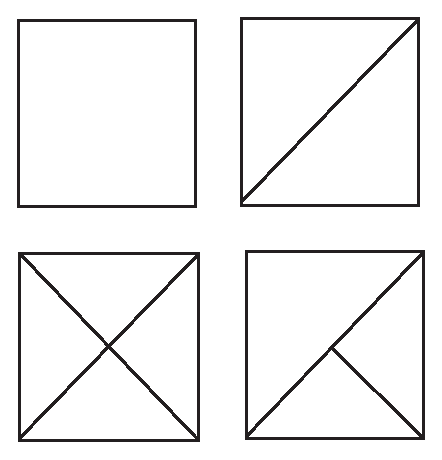
\includegraphics{PS/tame4circuit.eps}
        \caption{Tame $4$-circuits}
        \label{fig:fourcircuit}
    \end{figure}

    \item The degree of every vertex is at least $2$ and at most
    $6$.
    \label{definition:tame:degree}

    \item If a vertex is contained in an exceptional face,
        then the degree of the vertex is at most $5$.
    \label{definition:tame:degreeE}

    \item $$\sum_F c(len(F)) \ge 8,$$
    \label{definition:tame:score}


    \item There exists an admissible weight assignment
        of total weight less than the target, $\op{tgt}=14.8$.
    \label{definition:tame:squander}

    \item There are never two vertices of type $(4,0)$ that are
    adjacent to each other.
    \label{definition:tame:40}

\end{enumerate}
%
It follows from the definitions that the abstract vertex-edge
graph of $G$ has no loops or multiple joins.  Also, by
construction, every vertex lies in at least two faces. Property
\ref{definition:tame:score} implies that the graph has at least
        eight triangles.

\begin{remark}
We pause to review the strategy of the proof of the Kepler
conjecture as described in Section~\ref{sec:outline}. The
decomposition stars that violate the main inequality $\sigma(D)\ge
8\,\pt$ are said to contravene.  A plane graph is associated with
each contravening decomposition star.  These are the contravening
plane graphs. The main object of this paper is to prove that the
only two contravening graphs are $G_{fcc}$ and $G_{hcp}$, the graphs
associated with the face-centered cubic and hexagonal close
packings.

We have defined a set of plane graphs, called {\it tame graphs}. The
next \chap\ will give a classification of tame plane graphs. (There
are several thousand.) \Chap~\ref{sec:startame} gives a proof that
all contravening plane graphs are tame.  By the classification
result, this reduces the possible contravening graphs to an explicit
finite list.  Case-by-case linear programming arguments will show
that none of these tame plane graphs is a contravening graph (except
$G_{fcc}$ and $G_{hcp}$).  Having eliminated all possible graphs, we
arrive at the resolution of the Kepler conjecture.
\end{remark}




\chapter{Classification of Tame Plane Graphs}
    \label{sec:proof-classification}

\section{Statement of the Theorem}
\label{sec:classification}

A list of several thousand plane graphs appears at \cite{web}. The
following theorem is listed as one of the central claims in the
proof in Section~\ref{sec:logic}.

\begin{theorem}
\label{theorem:classification} Every tame plane graph is
isomorphic to a plane graph in this list.
\end{theorem}

The results of this section are not needed except in the proof of
Theorem \ref{theorem:classification}.

\smallskip

Computers are used to generate a list of all tame plane graphs and
to check them against the archive of tame plane graphs.  We will
describe a finite state machine that produces all tame plane
graphs. This machine is not particularly efficient, and so we also
include a description of pruning strategies that prevent a
combinatorial explosion of possibilities.


\section{Basic Definitions}

In order to describe how all tame plane graphs are generated, we
need to introduce {\it partial plane graphs}, that encode an
incompletely generated tame graph.  A partial plane graph is
itself a graph, but marked in such a way to indicate that it is in
a transitional state that will be used to generate further plane
graphs.

\begin{definition}
A {\it partial plane graph} is a plane graph with additional data:
every face is marked as ``complete'' or ``incomplete.'' We call a
face {\it complete\/} or {\it incomplete\/} according to the
markings. We require the following condition.
\begin{itemize}
  \item {\it No two incomplete faces share an edge.}
  \label{definition:partial (plane graph)}
\end{itemize}
\end{definition}

Each unmarked plane graph is identified with the marked plane
graph in which every face is complete. We represent a partial
plane graph graphically by deleting one face (the face at
infinity) and drawing the others and shading those that are
complete.

A {\it patch\/} is a partial plane graph $P$ with two
distinguished faces $F_1$ and $F_2$, such that the following hold.
\begin{itemize}
  \item Every vertex of $P$ lies in $F_1$ or $F_2$.
  \item The face $F_2$ is the only complete face.
  \item $F_1$ and $F_2$ share an edge.
  \item Every vertex of $F_2$ that is not in $F_1$
has degree $2$.
%
 \index{patch}
\end{itemize}

$F_1$ and $F_2$ will be referred to as the distinguished
incomplete and the distinguished complete faces, respectively.

Patches can be used to modify a partial plane graph as follows.
Let $F$ be an incomplete face of length $n$ in a partial plane
graph $G$. Let $P$ be a patch whose incomplete distinguished face
$F_1$ has length $n$. Replace $P$ with a properly isomorphic patch
$P'$ in which the image of $F_1$ is equal to $F^{op}$ and in which
no other vertex of $P'$ is a vertex of $G$. Then
    $$ G' = \{F' \in G\cup P' : F'\ne F^{op}, F'\ne F\}$$
is a partial plane graph. Intuitively, we cut away the faces $F$
and $F_1$ from their plane graphs, and glue the holes together
along the boundary (Figure \ref{fig:patching}). (It is immediate
that the Condition \ref{definition:partial (plane graph)} in the
definition of partial plane graphs is maintained by this process.)
There are $n$ distinct proper ways of identifying $F_1$ with
$F^{op}$ in this construction, and we let $\phi$ be this
identification. The isomorphism class of $G'$ is uniquely
determined by the isomorphism class of $G$, the isomorphism class
of $P$, and $\phi$ (ranging over proper bijections
$\phi:F_1\mapsto F^{op}$).
\begin{figure}[htb]
  \centering
  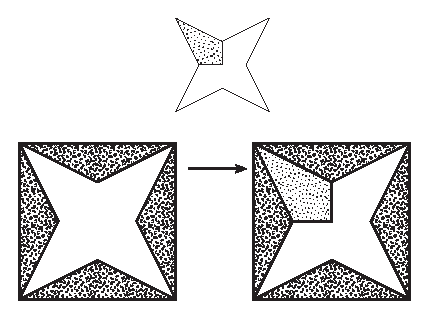
\includegraphics{PS/patching2.eps}
  \caption{Patching a plane graph}
  \label{fig:patching}
\end{figure}


\section{A Finite State Machine}

For a fixed $N$ we define a finite state machine as follows. The
states of the finite state machine are isomorphism classes of
partial plane graphs $G$ with at most $N$ vertices. The
transitions from one state $G$ to another are isomorphism classes
of pairs $(P,\phi)$ where $P$ is a patch, and $\phi$ pairs an
incomplete face of $G$ with the distinguished incomplete face of
$P$. However, we exclude a transition $(P,\phi)$ at a state if the
resulting partial plane graphs contains more than $N$ vertices.
Figure \ref{fig:patching} shows two states and a transition
between them.

The initial states $I_n$ of the finite state machine are defined
to be the isomorphism classes of partial plane graphs with two
faces:
    $$\{(1,2,\ldots,n),(n,n-1,\ldots,1)\}$$
where $n\le N$, one face is complete, and the other is incomplete.
In other words, they are patches with exactly two faces.

A terminal state of this finite state machine is one in which
every face is complete.  By construction, these are (isomorphism
classes of) plane graphs with at most $N$ vertices.

\begin{lemma}
    \label{lemma:reachable}
Let $G$ be a plane graph with at most $N$ vertices. Then its state
in the machine is reachable from an initial state through a series
of transitions.
\end{lemma}

\begin{proof}  Pick an face in $G$ of length $n$ and identify it with
the complete face in the initial state $I_n$. At any stage at
state $G'$, we have an identification of all of the vertices of
the plane graph $G'$ with some of the vertices of $G$, and an
identification of all of the complete faces of $G'$ with some of
the faces of $G$ (all faces of $G$ are complete). Pick an
incomplete face $F$ of $G'$ and an oriented edge along that face.
We let $F'$ be the complete face of $G$ with that edge, with the
same orientation on that edge as $F$. Create a patch with
distinguished faces $F_1 = F^{op}$ and $F_2 = F'$. ($F_1$ and
$F_2$ determine the patch up to isomorphism.) It is immediate that
the conditions defining a patch are fulfilled. Continue in this
way until a graph isomorphic to $G$ is reached.
\end{proof}

\begin{remark}
It is an elementary matter to generate all patches $P$ such that
the distinguished faces have given lengths $n$ and $m$. Patching
is also entirely algorithmic, and thus by following all paths
through the finite state machine, we obtain all plane graphs with
at most $N$ vertices.
\end{remark}

\section{Pruning Strategies}

Although we reach all graphs in this manner, it is not
computationally efficient. We introduce pruning strategies to
increase the efficiency of the search. We can terminate our search
along a path through the finite state machine, if we can
determine:
\begin{enumerate}
  \item Every terminal graph
along that path violates one of the defining properties of
tameness, or
    \label{enum:not-tame}
  \item An isomorphic terminal graph will be reached by
some other path that will not be terminated early.
    \label{enum:branch}
\end{enumerate}

Here are some pruning strategies of the first type
(\ref{enum:not-tame}). They are immediate consequences of the
conditions of the defining properties of tameness.

\begin{itemize}
  \item If the current state contains an incomplete face of length 3,
    then eliminate all transitions, except for the transition
    that carries the partial plane graph to a partial plane graph that
    is the same in all respects, except that the face has
    become complete.
  \item If the current state contains an incomplete face of length 4,
    then eliminate all transitions except those that lead to
    the possibilities of Section \ref{sec:graphproperty},
    Property \ref{definition:tame:4-circuit},
    where in Property \ref{definition:tame:4-circuit}
     each depicted face is interpreted
    as being complete.
  \item Remove all transitions with
    patches whose complete face has length greater than
    $8$.
  \item It is frequently possible to conclude from the examination of a partial
    plane graph that no matter what the terminal position,
    any admissible weight assignment will give total weight greater than
    the target $(\op{tgt}=14.8)$.  In such cases, all transitions out of the
    partial plane graph can be pruned.
\end{itemize}

    To take a simple example of the last item, we observe that weights are always
    nonnegative, and that the weight of a complete face of
    length $n$ is at least $d(n)$.  Thus, if there are complete
    faces $F_1,\ldots,F_k$ of lengths $n_1,\ldots,n_k$, then
     any admissible weight assignment has total weight at least
    $\sum_{i=1}^k d(n_i)$.  If this number is at least the
    target, then no transitions out of that state need be considered.

More generally, we can apply all of the inequalities in the
definition of admissible weight assignment to the complete portion
of the partial plane graph to obtain lower bounds.  However, we
must be careful, in applying Property
\ref{definition:admissible:excess} of admissible weight
assignments, because vertices that are not adjacent at an
intermediate state may become adjacent in the complete graph.
Also, vertices that do not lie together in a quadrilateral at an
intermediate state may do so in the complete graph.


Here are some pruning strategies of the second type
(\ref{enum:branch}).
\begin{itemize}
    \item At a given state it is enough to fix one incomplete face and
        one edge of that face and then to follow only the transitions that
        patch along that face and add a complete face along that
        edge. (This is seen from the proof of Lemma
        \ref{lemma:reachable}.)
    \item In leading out from the initial state $I_n$, it is enough
        to follow paths in which every added complete face has
        length at most $n$. (A graph with a face of length $m$,
        for $m>n$, will be also be found downstream from $I_m$.)
    \item Make a list of all type $(p,q)$ with $b(p,q)<\op{tgt}=14.8$.
    Remove the initial states $I_3$ and $I_4$, and create new initial states
    $I_{p,q}$  ($I_{p,q}'$, $I_{p,q}''$, etc.)
    in the finite state machine.  Define the state $I_{p,q}$ to be
    one consisting of $p+q+1$ faces, with $p$ complete triangles
    and $q$ complete quadrilaterals all meeting at a vertex
    (and one other incomplete face away from $v$).
    (If there is more than one way to arrange $p$ triangles and
    $q$ quadrilaterals, create states $I_{p,q}$, $I'_{p,q}$,
    $I''_{p,q}$, for each possibility.  See Figure \ref{fig:states}.)
    Put a linear order on states $I_{p,q}$.  In state transitions
    downstream from $I_{p,q}$ disallow any transition that creates
    a vertex of type $(p',q')$, for any $(p',q')$ preceding $(p,q)$
    in the imposed linear order.
\end{itemize}
\begin{figure}[htb]
  \centering
  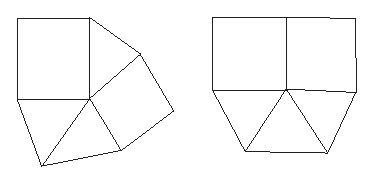
\includegraphics{PS/Ipq.eps}
  \caption{States $I_{3,2}$ and $I_{3,2}'$}
  \label{fig:states}
\end{figure}

This last pruning strategy is justified by the following lemma,
which classifies vertices of type $(p,q)$.

\begin{lemma}
Let $A$ and $B$ be triangular or quadrilateral faces that have at
least $2$ vertices in common in a tame graph. Then the faces have
exactly two vertices in common, and an edge is shared by the two
faces.
\end{lemma}

\begin{proof}
Exercise.  Some of the configurations that must be ruled out are
shown in Figure \ref{fig:nonexistant}.  Some properties that are
particularly useful for the exercise are Properties
\ref{definition:tame:3-circuit} and
\ref{definition:tame:4-circuit} of tameness, and Property
\ref{admissible:b} of admissibility.
\end{proof}
\begin{figure}[htb]
  \centering
  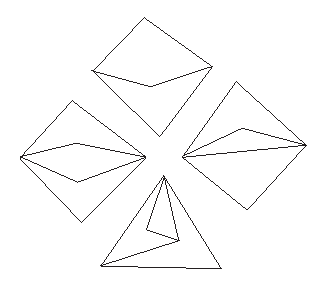
\includegraphics{PS/impossible.eps}
  \caption{Some impossibilities}
  \label{fig:nonexistant}
\end{figure}

Once a terminal position is reached it is checked to see whether
it satisfies all the properties of tameness.

Duplication is removed among isomorphic terminal plane graphs. It
is not an entirely trivial procedure for the computer to determine
whether there exists an isomorphism between two plane graphs. This
is accomplished by computing a numerical invariant of a vertex
that depends only on the local structure of the vertex. If two
plane graphs are properly isomorphic then the numerical invariant
is the same at vertices that correspond under the proper
isomorphism.  If two graphs have the same number of vertices with
the same numerical invariants, they become candidates for an
isomorphism.  All possible numerical-invariant preserving
bijections are attempted until an proper isomorphism is found, or
until it is found that none exist. If there is no proper
isomorphism, the same procedure is applied to the opposite plane
graph to find any possible orientation-reversing isomorphism.

This same isomorphism-producing algorithm is used to match each
terminal graph with a graph in the archive.  It is found that each
terminal graph matches with one in the archive. (The archive was
originally obtained by running the finite state machine and making
a list of all the terminal states up to isomorphism that satisfy
the given conditions.)

In this way Theorem \ref{theorem:classification} is proved.

\chapter{Contravening Graphs}
    \label{sec:startame}

We have seen that a system of points and arcs on the unit sphere
can be associated with a decomposition star $D$.  The points are
the radial projections of the vertices of $U(D)$ (those at
distance at most $2t_0=2.51$ from the origin).  The arcs are the
radial projections of edges between $v,w\in U(D)$, where
$|v-w|\le2t_0$.  If we consider this collection of arcs
combinatorially as a graph, then it is not always true that these
arcs form a plane graph in the restrictive sense of
\Chap~\ref{sec:def-and-class}.

The purpose of this \chap\ is to show that if the original
decomposition star contravenes, then minor modifications can be
made to the system of arcs graph so that the resulting
combinatorial graph has the structure of a plane graph in the
sense of \Chap~\ref{sec:def-and-class}. These plane graphs are
called contravening plane graphs, or simply contravening graphs.


\section{A Review of Earlier Results}
    \label{sec:star-review}

\shortversion{In this \chap, we will make use of several results
that appear in the unabridged version of this paper.  In this
section, we collect together the most important of these results.
}

Let $\zeta = 1/(2\arctan(\sqrt{2}/5))$. Let $\sol(R)$ denote the
solid angle of a standard region $R$.  We write $\tau_R$ for the
following modification of $\sigma_R$:
%
 \index{ZZdzeta@$\zeta= 1/(2\arctan(\sqrt{2}/5))$}
 \index{sol@$\sol(R)$}
 \index{ZZtau@$\tau_R$}
 \index{ZZtau@$\tau$}
    \begin{equation}
    \tau_R(D) = \sol(R)\zeta\pt - \sigma_R(D)
    \label{eqn:tauR-def}
    \end{equation}
and
    \begin{equation}
    \tau(D) = \sum\tau_R(D) = 4\pi\zeta\pt - \sigma(D).
    \label{eqn:tau-def}
    \end{equation}
Since $4\pi\zeta\pt$ is a constant, $\tau$ and $\sigma$ contain
the same information, but $\tau$ is often more convenient to work
with. A contravening decomposition star satisfies
    \begin{equation}
    \tau(D) \le 4\pi\zeta\pt -8\,\pt = (4\pi\zeta-8)\pt.
    \label{eqn:tau-sig}
    \end{equation}
The constant $\squander$  (and its upper bound $\op{tgt}\,\pt$
where $\op{tgt}=14.8$) will occur repeatedly in the discussion
that follows.

Recall that a standard cluster is a pair $(R,D)$ consisting of a
decomposition star $D$ and one of its standard regions $R$. If $F$
is a finite set (or finite union) of standard regions, let
    \begin{equation}
    \sigma_F(D) = \sum_R \sigma_R(D),\quad \tau_F(D) =
    \sum_R\tau_R(D),
    \label{eqn:sig-F}
    \end{equation}
where the sum runs over all the standard regions in $F$.  When the
sum runs over all standard regions, we have
    \begin{equation}
    \sigma(D) = \sum\sigma_R(D),\quad \tau(D) =\sum\tau_R(D).
    \label{eqn:sig-all}
    \end{equation}

A natural number $n(R)$ is associated with each standard region.
If the boundary of that region is a simple polygon, then $n(R)$ is
the number of sides.   If the boundary consists of $k$ disjoint
simple polygons, with $n_1,\ldots,n_k$ sides then
    $$n(R) = n_1+\cdots+n_k + 2(k-1).$$

\begin{lemma}\label{cor:std-aggregate-list:bis}
Let $R$ be a standard region in a contravening decomposition star
$D$.  The boundary of $R$ is a simple polygon with at most $8$
edges, or one of the configurations of
Figure~\ref{fig:aggregates}.
\end{lemma}

\begin{proof} \shortversion{See \cite{KC}.}
    \longversion{This is Theorem~\ref{thm:the-main-theorem} and
    Corollary~\ref{cor:std-aggregate-list}.}
%Corollary~\ref{cor:std-aggregate-list})
\end{proof}

\begin{figure}[htb]
  \centering
  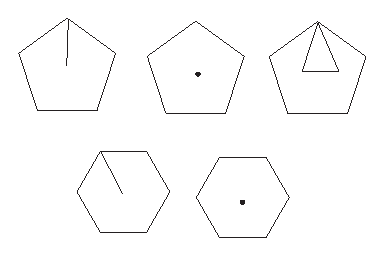
\includegraphics{PS/nonpolygon.eps}
  \caption{Non-polygonal standard regions ($n(R)=7,7,8,8,8$)}
  \label{fig:aggregates}
\end{figure}

\begin{lemma} \label{lemma:sn-tn}
Let $R$ be a standard region.  We have
$\tau_R(D)\ge t_n$, where $n=n(R)$, and
    $$
    \begin{array}{lllll}
    t_3&=0,\quad t_4&=0.1317,\quad t_5=0.27113,\quad
    t_6&=0.41056\quad t_7&=0.54999,\quad t_8=0.6045.
    \end{array}
    $$
Furthermore, $\sigma_R(D)\le s_n$, for $5\le n\le 8$, where
    $$
    s_3=1\,\pt,\quad s_4=0,\quad
    s_5=-0.05704,\quad s_6=-0.11408,\quad
    s_7=-0.17112,\quad s_8=-0.22816.
    $$
\end{lemma}

\begin{proof} \shortversion{\cite{KC}.}
    \longversion{This is Theorem~\ref{thm:the-main-theorem}.}
\end{proof}


\begin{lemma} \label{lemma:s9-t9:bis}
Let $F$ be a set of standard regions bounded by a simple polygon
with at most $9$ edges.  Assume  that
    $$\sigma_F(D) \le s_9\quad\text{and }\tau_F(D)\ge t_9,$$
where $s_9=-0.1972$ and $t_9=0.6978$.  Then $D$ does not
contravene.
\end{lemma}

\begin{proof} \shortversion{\cite{KC}.}
    \longversion{This is Section~\ref{sec:nonagon}.}
\end{proof}

\begin{lemma}  \label{lemma:0pt-1pt}
Let $(R,D)$ be a standard cluster.  If $R$ is a triangular
region, then
    $$\sigma_R(D)\le1\,\pt.$$
If $R$ is not a triangular region, then
    $$\sigma_R(D)\le 0.$$
\end{lemma}

\begin{proof} See Lemma~\ref{lemma:1pt} and Theorem~\ref{lemma:quad0}.
\end{proof}

\begin{lemma}\label{lemma:roger0:bis}
    %proclaim{Lemma 3.1}
    \oldlabel{part3.3.1}
    $\tau_R(D)\ge 0$, for all standard clusters $R$.
\end{lemma}

\begin{proof}  \shortversion{\cite{KC}.}
    \longversion{This is Lemma~\ref{lemma:roger0}.}
\end{proof}



Recall that $v$ has {\it type\/} $(p,q)$ if every standard region
with a vertex at  $v$ is a triangle or quadrilateral, and if there
are exactly $p$ triangular faces and $q$ quadrilateral faces that
meet at $v$ (see Definition~\ref{definition:type}).  We write
$(p_v,q_v)$ for the type of $v$. Define constants $\tlp(p,q)/\pt$
by Table~\ref{eqn:old5.1:bis}. The entries marked with an asterisk
will not be needed.
%
 \index{type (of a vertex)}
 \index{ZZtauLP@$\tlp(p,q)$}

\begin{equation}
\vbox{\offinterlineskip \hrule
\halign{&\vrule#&\strut\ \hfil#\hfil\ \cr   % "\ " was quad
height 7pt&\omit&&\omit&&\omit&&\omit&&\omit&&\omit&&\omit&\cr
&\hfil $\tlp(p,q)/\pt$\hfil
        &&\hfil $q=0$\hfil
        &&\hfil1\hfil
        &&\hfil2\hfil
        &&\hfil3\hfil
        &&\hfil4\hfil
        &&\hfil5\hfil&
\cr height 7pt&\omit&&\omit&&\omit&&\omit&&\omit&&\omit&&\omit&\cr
\noalign{\hrule}
height7pt&\omit&&\omit&&\omit&&\omit&&\omit&&\omit&&\omit&\cr
&$p=0$&& *&& *&& 15.18&& 7.135&& 10.6497&& 22.27&\cr &1&&    *&&
*&&  6.95&& 7.135&&17.62  && 32.3&\cr &2&&    *&&
8.5&&4.756&&12.9814&&*&&*&\cr &3&& *&&
3.6426&&8.334&&20.9&&*&&*&\cr
&4&&4.1396&&3.7812&&16.11&&*&&*&&*&\cr
&5&&0.55&&11.22&&*&&*&&*&&*&\cr &6&&6.339&&*&&*&&*&&*&&*&\cr
&7&&14.76&&*&&*&&*&&*&&*&\cr
height7pt&\omit&&\omit&&\omit&&\omit&&\omit&&\omit&&\omit&\cr}
\hrule }
    %oldtag 5.1
    \label{eqn:old5.1:bis}
\end{equation}

\begin{lemma} \label{lemma:pq:bis} %{Proposition 5.2}
Let $S_1,\ldots,S_p$ and $R_1,\ldots,R_q$ be the tetrahedra and
quad clusters around a vertex of type $(p,q)$. Consider the
constants of Table~\ref{eqn:old5.1:bis}.  We have
    $$
    \begin{array}{lll}
    &\sum^p\tau(S_i) + \sum^q\tau(R_i) \ge \tlp(p,q).\\
    \end{array}
    $$
\end{lemma}

\begin{proof} \shortversion{\cite{KC}.}
    \longversion{This is Lemma~\ref{lemma:pq}.}
\end{proof}

\begin{lemma} \label{lemma:0.55:bis} %proclaim{Lemma 5.3}
Let $v_1,\ldots, v_k$, for some $k\le 4$, be distinct vertices of
type $(5,0)$.  Let $S_1,\ldots, S_r$ be quasi-regular tetrahedra
around the edges $(0,v_i)$, for $i\le k$. Then
    $$
    \sum_{i=1}^r \tau(S_i)> 0.55k\,\pt,
    $$
and
    $$\sum_{i=1}^r \sigma(S_i) < r\,\pt - 0.48k\,\pt.$$
\end{lemma}

\begin{proof} \shortversion{\cite{KC}.}
    \longversion{This is Lemma~\ref{lemma:0.55}.}
\end{proof}

\begin{lemma}\label{lemma:pq-types:bis} %\proclaim{Lemma 6.2}
Let $D$ be a contravening decomposition star.  If the type of the
vertex is $(p,q,r)$ with $r=0$, then $(p,q)$ must be one of the
following:
    $$\{
        (6,0),(5,0),(4,0),
        (5,1),(4,1),(3,1),(2,1),
        (3,2),(2,2),(1,2),
        (2,3),(1,3),(0,3),(0,4)\}.$$
\end{lemma}

\begin{proof} \shortversion{\cite{KC}.}
    \longversion{This is Lemma~\ref{lemma:pq-types} and Lemma~\ref{lemma:70}.}
\end{proof}

\begin{lemma}
        \label{lemma:no-enclosed-tri:bis}
        A triangular standard region does not contain any enclosed
        vertices.
\end{lemma}

\begin{proof}
    This fact is proved in \cite[Lemma~3.7]{part1}.
\end{proof}

\begin{lemma}\label{lemma:enclosed:bis} % {Lemma 2.2}
A quadrilateral region does not enclose any vertices of height at
most $2t_0$.
\end{lemma}

\begin{proof} \shortversion{\cite{KC}.}
    \longversion{This is Lemma~\ref{lemma:enclosed}.}
\end{proof}

\begin{lemma}\label{lemma:no-2}
Let $F$ be a union of standard regions.    Suppose that the
boundary of $F$ consists of $4$ edges. Suppose that the area of
$F$ is at most $2\pi$.  Then there is at most one enclosed vertex
over $F$.
\end{lemma}

\begin{proof} This is \cite[Prop.~4.2]{part1}.
\end{proof}

\begin{lemma}\label{lemma:11.16:bis}
Let $F$ be the union of two standard regions, a triangular region
and a pentagonal region that meet at a vertex of type $(1,0,1)$ as
shown in Figure~\ref{fig:no4circuit:bis}.  Then
    $$\tau_F(D) \ge 11.16\,\pt.$$
\end{lemma}

\begin{proof} \shortversion{\cite{KC}.}
    \longversion{This is Lemma~\ref{lemma:11.16}.}
\end{proof}

\begin{figure}[htb]
  \centering
  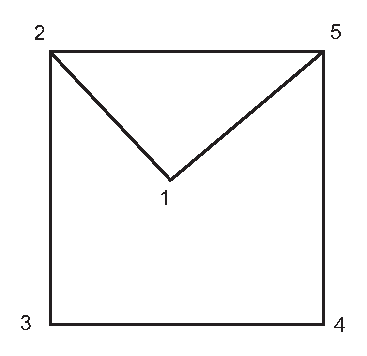
\includegraphics{PS/no4circuit.eps}
  \caption{A $4$-circuit}
  \label{fig:no4circuit:bis}
\end{figure}

%\begin{lemma}\label{lemma:5.66}
%Let $R$ be a pentagonal standard region.  Suppose that one of its
%angles is at most $1.32$.  Then
%    $$\tau_R(D)\ge 5.66\,\pt.$$
%\end{lemma}
%
%\begin{proof}
%\end{proof}

\begin{lemma}\label{lemma:1.47}
Let $R$ be an exceptional standard region.  Suppose that $R$ has $r$
different interior angles that are pairwise nonadjacent and such
that each is at most $1.32$.  Then
    $$\tau_R(D) \ge t_n + r (1.47)\,\pt.$$
\end{lemma}

\begin{proof} \shortversion{\cite{KC}.}
    \longversion{This is Remark~\ref{remark:1.47}.}
\end{proof}

\begin{lemma} \label{lemma:0.8638}
Every interior angle of every standard region is at least
$0.8638$. Every interior angle of every standard region that is
not a triangle is at least $1.153$
\end{lemma}
 %
 \index{ZZZZ1.153@$1.153$}
 \index{ZZZZ0.8638@$0.8638$}

\begin{proof}  \calc{208809199} and \calc{853728973-1}.
\end{proof}

\begin{definition}
The {\it central vertex\/} of a flat quarter is defined to be the
one that does not lie on the triangle formed by the origin and the
diagonal.
%
 \index{central (vertex)}
\end{definition}

\begin{lemma}\label{lemma:1.32:bis}
If the interior angle at a corner $v$ of a non-triangular standard
region is at most $1.32$, then there is a flat quarter over $R$
whose central vertex is $v$.
\end{lemma}

\begin{proof} \shortversion{\cite{KC}.}
    \longversion{This is Lemma~\ref{lemma:1.32}.}
\end{proof}



\section{Contravening Plane Graphs defined}
\label{sec:stargraph}

A plane graph $G$ is attached to every contravening decomposition
star as follows.  From the decomposition star $D$, it is possible
to determine the coordinates of the set $U(D)$ of vertices at
distance at most $2t_0 $ from the origin.

If we draw a geodesic arc on the unit sphere at the origin with
endpoints at the radial projections of $v_1$ and $v_2$ for every
pair of vertices $v_1$, $v_2\in U(D)$ such that $|v_1|, |v_2|,
|v_1-v_2|\le 2t_0 $, we obtain a plane graph that breaks the unit
sphere into standard regions. (The arcs do not meet except at
endpoints by Lemma~\ref{lemma:2t0-doesnt-pass-through}.)
%Each
%standard region is defined as the closure in the unit sphere of a
%connected component of the unit sphere with all arcs removed.

For a given standard region, we consider the arcs forming its
boundary together with the arcs that are internal to the standard
region.  We consider the points on the unit sphere formed by the
endpoints of the arcs, together with the radial projections to the
unit sphere of vertices in $U$ whose radial projection lies in the
interior of the region.

\begin{remark}
The system of arcs and vertices associated with a standard region
in a contravening example must be a polygon, or one of the
configurations of Figure~\ref{fig:aggregates} (see
Lemma~\ref{cor:std-aggregate-list:bis}).
\end{remark}


\begin{remark} \label{remark:tri-pent}
Observe that one case of Figure~\ref{fig:aggregates} is bounded by
a triangle and a pentagon, and that the others are bounded by a
polygon. Replacing the triangle-pentagon arrangement with the
bounding pentagon and replacing the others with the bounding
polygon, we obtain a partition of the sphere into simple polygons.
Each of these polygons is a single standard region, except in the
triangle-pentagon case (Figure~\ref{fig:tri-pent}), which is a
union of two standard regions (a triangle and a eight-sided
region).
\end{remark}
\begin{figure}[htb]
  \centering
  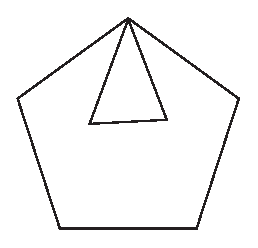
\includegraphics{PS/tripent.eps}
  \caption{An aggregate forming a pentagon}
  \label{fig:tri-pent}
\end{figure}

\begin{remark}\label{remark:degree6}
To simplify further, if we have an arrangement of six standard
regions around a vertex formed from five triangles and one
pentagon, we replace it with the bounding octagon (or hexagon).
See Figure~\ref{fig:degree6}.  (It will be shown in
Lemma~\ref{lemma:deg5} that there is at most one such
configuration in the standard decomposition of a contravening
decomposition star, so we will not worry here about how to treat
the case of two overlapping configurations of this sort.)
\end{remark}
\begin{figure}[htb]
  \centering
  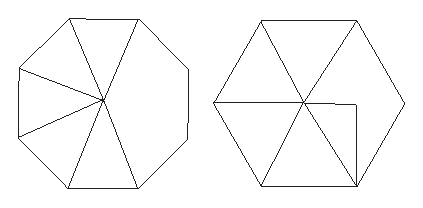
\includegraphics{PS/degree6.eps}
  \caption{Degree $6$ aggregates}
  \label{fig:degree6}
\end{figure}

In summary, we have a plane graph that is approximately that given
by the standard regions of the decomposition star, but simplified
to a bounding polygon when one of the configurations of Remarks
\ref{remark:tri-pent} and \ref{remark:degree6} occur.  We refer to
the combination of standard regions into a single face of the
graph as {\it aggregation}.  We call it the plane graph $G = G(D)$
attached to a contravening decomposition star $D$.
%
 \index{aggregation}

Proposition \ref{prop:nonempty} will show the vertex set $U$ is
nonempty and that the graph $G(D)$ is nonempty.

When we refer to the plane graph in this manner, we mean the
combinatorial plane graph as opposed to the embedded metric graph
on the unit sphere formed from the system of geodesic arcs.  Given
a vertex $v$ in $G(D)$, there is a uniquely determined vertex
$v(D)$ of $U(D)$ whose radial projection to the unit sphere
determines $v$.  We call $v(D)$ the {\it corner} in $U(D)$ over
$v$.
%
 \index{corner}

By construction, the plane graphs associated with a decomposition
star do not have loops or multiple joins.  In fact, the edges of
$G(D)$ are defined by triangles whose sides vary between lengths
$2$ and $2t_0 $. The angles of such a triangle are strictly less
than $\pi$.  This implies that the edges of the metric graph on
the unit sphere always have arc-length strictly less than $\pi$.
In particular, the endpoints are never antipodal.  A loop on the
combinatorial graph corresponds to a edge on the metric graph that
is a closed geodesic.  A multiple join on the combinatorial graph
corresponds on the metric graph to a pair of points joined by
multiple minimal geodesics, that is, a pair of antipodal points on
the sphere.  By the arc-length constraints on edges in the metric
graph, there are no loops or multiple joins in the combinatorial
graph $G(D)$.

In Definition \ref{definition:tame}, a plane graph satisfying a
certain restrictive set of properties is said to be {\it tame}. If
a plane graph $G(D)$ is associated with a contravening
decomposition star $D$, we call $G(D)$ a {\it contravening plane
graph}.
%
 \index{contravening plane graph}

\begin{theorem} \label{theorem:contravene}  Let $D$ be a
contravening decomposition star.  Then its plane graph $G(D)$ is
tame.
\end{theorem}

This theorem is one of the main steps in the proof of the Kepler
conjecture. It is advanced as one of the central claims in
Section~\ref{sec:logic}.  Its proof occupies
\Chaps~\ref{sec:contraproof} and \ref{sec:weight}. In Theorem
\ref{theorem:classification}, the tame graphs  are classified up to
isomorphism. As a corollary, we have an explicit list of graphs that
contains all contravening plane graphs.


\chapter{Contravention is tame}
    \label{sec:contraproof}

This section begins the proof of Theorem \ref{theorem:contravene}
(contravening graphs are tame). To prove Theorem
\ref{theorem:contravene}, it is enough to show that each defining
property of tameness is satisfied for every contravening graph.
This is the substance of results in the following sections. The
proof continues through the end of \Chap~\ref{sec:weight}. This
\chap\ verifies all the properties of tameness, except for the
last one (weight assignments).

\section{First Properties}

This section verifies Properties 1, 2, 4, and 8 of tameness.  First,
we prove the promised nondegeneracy result.

\begin{proposition}
\label{prop:nonempty} The construction of Section
\ref{sec:stargraph} associates a (nonempty) plane graph with at
least two faces to every decomposition star $D$ with
$\sigma(D)>0$.
\end{proposition}

\begin{proof}
First we show that decomposition stars with $\sigma(D)>0$ have
nonempty vertex sets $U$. (Recall that $U$ is the set of vertices
of distance at most $2t_0$ from the center).  The vertices of $U$
are used in \Chaps~\ref{sec:construction} and \ref{sec:vcells} to
create all of the structural features of the decomposition star:
quasi-regular tetrahedra, quarters, and so forth. If $U$ is empty,
the $V$-cell is a solid containing the ball $B(t_0)$ of radius
$t_0$, and $\sigma(D)$ satisfies
    $$
    \begin{array}{lll}
    \sigma(D) &= \vor(D)\\
              & = -4\doct \op{vol}(\op{VC}(D)) + 4\pi/3 \\
              &< -4\doct\op{vol}(B(t_0)) + 4\pi/3
              &< 0.
    \end{array}
    $$
By hypothesis, $\sigma(D)>0$.  So $U$ is not empty.

Equation~\ref{eqn:sig-all} shows that the function $\sigma$ can be
expressed as a sum of terms $\sigma_R$ indexed by the standard
regions $R$. It is proved in Theorem~\ref{lemma:quad0} that
$\sigma_R\le0$, unless $R$ is a triangle. Thus, a decomposition
star with positive $\sigma(D)$ must have at least one triangle.
Its complement contains a second standard region. Even after we
form aggregates of distinct standard regions to form the
simplified plane graph (Remarks \ref{remark:tri-pent} and
\ref{remark:degree6}), there certainly remain at least two faces.
\end{proof}

\begin{proposition} The plane graph of a contravening decomposition
star satisfies Property \ref{definition:tame:length} of tameness:
The length of each face is at least $3$ and at most $8$.
\end{proposition}

\begin{proof} By the construction of the graph, each face has at
least three edges.  The upper bound of $8$ edges is
Lemma~\ref{cor:std-aggregate-list:bis}.  Note that the aggregates of
Remarks~\ref{remark:degree6} and \ref{remark:tri-pent} have between
$5$ and $8$ edges.
\end{proof}

\begin{proposition} The plane graph of a contravening decomposition star
satisfies Property \ref{definition:tame:3-circuit} of tameness:
Every $3$-circuit is a face or the opposite of a face.
\end{proposition}

\begin{proof}
The simplifications of the plane graph in Remarks
\ref{remark:tri-pent} and \ref{remark:degree6}  do not produce any
new $3$-circuits. (See the accompanying figures.) The result is
Lemma~\ref{lemma:no-enclosed-tri:bis}.
\end{proof}

\begin{proposition} Contravening graphs satisfy Property
\ref{definition:tame:degree} of tameness: The degree of every
vertex is at least $2$ and at most $6$.
\end{proposition}

\begin{proof}
The statement that degrees are at least $2$ trivially follows
because each vertex lies on at least one polygon, with two edges
at that vertex.

If the type is $(p,q)$, then the impossibility of a vertex of
degree $7$ or more is found in Lemma~\ref{lemma:pq-types:bis}.  If
the type is $(p,q,r)$, with $r\ge1$, then Lemma~\ref{lemma:0.8638}
shows that the interior angles of the standard regions cannot sum
to $2\pi$:
    $$6 (0.8638) + 1.153 > 2\pi.$$
\end{proof}

\begin{proposition} Contravening graphs satisfy Property
\ref{definition:tame:40} of tameness: There are never two vertices
of type $(4,0)$ that are adjacent to each other. \end{proposition}

\begin{proof}
This is proved in \cite[4.2]{part1}.
\end{proof}

%\chapter{More Tame Properties} %section
%    \label{sec:moretame}



\section{Computer Calculations and Their Consequences}

This section continues in the proof that all contravening plane
graphs are tame.  The next few sections verify Properties 6, 5,
and then 3 of tameness.

In this \chap, we  rely on some inequalities that are not proved
in this paper.  Recall from Section~\ref{sec:bounds-simplex} that
there is an archive of hundreds of inequalities that have been
proved by computer. This full archive appears in \cite{web}.  The
justification of these inequalities appears in the same archive.
(The proofs of these inequalities were executed by computer.) Each
inequality carries a nine digit identifying number.  To invoke an
inequality, we state it precisely, and give its identifying
number, e.g. \calc{123456789}.

%\longversion{In fact, there are two groups of inequalities in the
%archive. One group consists of inequalities whose proofs were
%fully automated by computer.  Another group contains inequalities
%that must be manipulated in some simple way before they can be
%proved by computer.  Usually, these manipulations make use of
%monotonicity of a function known to be monotonic.  In other cases,
%they are formal consequences of other inequalities that have
%already been proved by computer, so that there is no need for a
%separate verification of the inequality.  In each case, the
%inequality is accompanied by a justification. Inequalities in this
%second group also carry a nine digit identifying number, e.g.
%\conseq{123456789}.}

To use these inequalities systematically, we combine inequalities
into linear programs and solve the linear programs on computer. At
first, our use of linear programs will be light, but our reliance
will become progressively strong as the argument develops.

To start out, we will make use of several calculations\footnote{The
sequence of five inequalities starting with \calc{927432550},
Lemma~\ref{lemma:roger0:bis}, and for quads \calc{310151857},
\calc{655029773}, \calc{73283761}, \calc{15141595},
\calc{574391221}, \calc{396281725}}
%the sequence of six starting \cite[Theorem~4.1]{part 3}.}
%This is SPIII, theorem 4.1 in the 1998 and 2002 versions
%SPIII 10. Calcs. Group 3.
%\footnote{\calc{\ref{calc:qrtet}} and \calc{\ref{calc:quad-bounds}}}.
%These inequalities
that give lower bounds on $\tau_R(D)$ when $R$ is a triangle or
quadrilateral. To obtain lower bounds through linear programming,
we take a linear relaxation. Specifically, we introduce a linear
variable for each function $\tau_R$ and a linear variable for each
interior angle $\alpha_R$. We substitute these linear variables
for the nonlinear functions $\tau_R(D)$ and nonlinear interior
angle function into the given inequalities. Under these
substitutions, the inequalities become linear.   Given $p$
triangles and $q$ quadrilaterals at a vertex, we have the linear
program to minimize the sum of the (linear variables associated
with) $\tau_R(D)$ subject to the constraint that the (linear
variables associated with the)  angles at the vertex sum to at
most $d$. Linear programming yields\footnote{Although they are
closely related, the function $\tauLP$ of three arguments
introduced here is distinct from the function of two variables of
the same name that is introduced in
Section~\ref{sec:star-review}.} a lower bound $\tauLP(p,q,d)$ to
this minimization problem. This gives  a lower bound to the
corresponding constrained sum of nonlinear functions $\tau_R$.

Similarly, another group of inequalities%
\footnote{ \calc{539256862}, \calc{864218323}, \calc{776305271}, and
for quads \calc{310151857}, \calc{655029773}, \calc{73283761},
\calc{15141595}, \calc{574391221}, \calc{396281725}}
% and \cite[Theorem~4.1]{part 3}.} %
% This is SPIII, theorem 4.1 in the 1998 and 2002 versions
% SPIII 10. Calcs. Group 3.
yield upper bounds $\sLP(p,q,d)$ on the sum of $p+q$ functions
$\sigma_R$, with $p$ standard regions $R$ that are triangular, and
another $q$ that are quadrilateral. These linear programs find
their first application in the proof of the following proposition.



\section{Linear Programs} %subsection
\label{sec:2.2}  To continue with the proof that contravening
plane graphs are tame, we need to introduce some more notation and
methods.

%The function $\sigma$ can be written is a sum of functions on the
%space of decomposition stars, indexed by standard regions.  (See
%Equation~\ref{eqn:sig-all} of Section~\ref{sec:star-review}.)
%Write $\sigma_R$ for the term indexed by the standard region $R$.
%Then
%    $$\sigma(D) = \sum_R \sigma_R(D),$$
%for every decomposition star.

If $F$ is a face of $G(D)$, let
    $$\sigma_F(D) = \sum \sigma_R(D),$$
where the sum runs over the set of standard regions associated
with $F$.  This sum reduces to a single term unless $F$ is an
aggregate in the sense of Remarks~\ref{remark:degree6} and
\ref{remark:tri-pent}.


\begin{lemma}
    The plane graph of a contravening decomposition star satisfies
    Property \ref{definition:tame:score} of tameness:
    $$\sum_F c(len(F)) \ge 8.$$
\end{lemma}

\begin{proof}
We will show that
    \begin{equation}
    c(len(F))\,\pt \ge \sigma_F(D)
    \label{eqn:sigma}
    \end{equation}
    Assuming this, the result follows for contravening
    stars $D$:
    $$
    \begin{array}{lll}
        \sum_F c(len(F)) \,\pt &\ge \sum_F \sigma_F(D) \\
            &= \sigma(D) \ge 8\,\pt.
    \end{array}
    $$

We consider three cases for Inequality \ref{eqn:sigma}. In the
first case, assume that the face $F$ corresponds to exactly one
standard region in the decomposition star.  In this case,
Inequality \ref{eqn:sigma} follows directly from the bounds of
Lemma~\ref{lemma:sn-tn}:
    $$\sigma_F(D)\le s_n \le c(n)\,\pt.$$

In the second case, assume we are in the context of a pentagon $F$
formed in Remark~\ref{remark:tri-pent}.  Then, again by
Theorem~\ref{lemma:sn-tn}, we have
$$\sigma_F(D) \le s_3+s_8\le (c(3)+c(8))\,\pt \le c(5)\,\pt.$$
(Just examine the constants $c(k)$.)

In the third case, we consider the situation of Remark
\ref{remark:degree6}.  The six standard regions give
$$\sigma_F(D)\le s_5+\sLP(5,0,2\pi-1.153)< c(8)\,\pt.$$
The constant $1.153$ comes from Lemma~\ref{lemma:0.8638}.
\end{proof}

\begin{proposition}
    \label{proposition:wttau}
    Let $F$ be a face of a contravening plane graph $G(D)$.
    Then
    $$\tau_F(D) \ge d(len(F))\pt.$$
\end{proposition}

\begin{proof} Similar.
\end{proof}

\begin{lemma}  If $v$  is a vertex of an exceptional standard region,
and if there are $6$ standard regions meeting at $v$, then the
exceptional region is a pentagonal region and the other $5$
standard regions are triangular.
\end{lemma}

%\begin{lemma}  Suppose that there are six or more standard
%regions around a vertex.  Then either (1) all the regions are
%triangles and the vertex has type $(6,0)$, or
%(2) there are five triangles, no quadrilaterals,
%and one exceptional face.
%\end{lemma}

\begin{proof}
%Assume (1) does not occur.
% If there are no  standard regions of length at least $5$ at the
%vertex, then the result follows from the inequalities of \cite[5.2]{pat3}
%and \cite[4.5]{pat4}:
%$$\tau(D^*)> t_5 + \min_{p+2q>6}
%    \tau(p,q)\ge 4.896\,\pt+11.22\,\pt \ge \squander.$$
%Without loss of generality, we assume there is an exceptional face
%at the vertex.
There are several cases according to the number $k$ of triangular
regions at the vertex.

{\bf($k\le2$)} If there are at least four non-triangular regions
at the vertex, then the sum of interior angles around the vertex
is at least $4(1.153)+2(0.8638)>2\pi$, which is impossible.  (See
Lemma~\ref{lemma:0.8638}.)

{\bf($k=3$)} If there are three non-triangular regions at the
vertex, then $\tau(D)$ is at least
$2t_4+t_5+\tauLP(3,0,2\pi-3(1.153))>\squander$.

{\bf($k=4$)} If there are two exceptional regions at the vertex,
then $\tau(D)$ is at least
$2t_5+\tauLP(4,0,2\pi-2(1.153))>\squander$.

If there are two non-triangular regions at the vertex, then
$\tau(D)$ is at least  $t_5+\tauLP(4,1,2\pi-1.153)>\squander$.

{\bf($k=5$)} We are left with the case of five triangular regions
and one exceptional region.

When there is an exceptional standard region at a vertex of degree
six, we claim that the exceptional region must be a pentagon. If
the region is a heptagon or more, then $\tau(D)$ is at least
$t_7+\tauLP(5,0,2\pi-1.153) > \squander$.

If the standard region is a hexagon, then $\tau(D)$ is at least
$t_6 + \tauLP(5,0,2\pi-1.153) > t_9$. Also,
$s_6+\sLP(5,0,2\pi-1.153) < s_9$. The aggregate of the six
standard regions is $9$-sided.  Lemma~\ref{lemma:s9-t9:bis} gives
the bound of $8\,\pt$.
\end{proof}


\begin{lemma}
    \label{lemma:aggregate6}
    Consider the standard regions of a contravening star $D$.
    \begin{enumerate}
    \item If a vertex of a pentagonal standard region has degree six,
    then the aggregate $F$ of the six faces satisfies
            $$
            \begin{array}{lll}
            \sigma_F(D) < s_8,\\
            \tau_F(D) > t_8.
            \end{array}
            $$
    \item There are at most two vertices of standard regions
    that lie on six standard regions.   If
        there are two, then they are nonadjacent vertices on a
        pentagon, as shown in Figure \ref{fig:doubledegree6}.
    \end{enumerate}
\end{lemma}
\begin{figure}[htb]
  \centering
  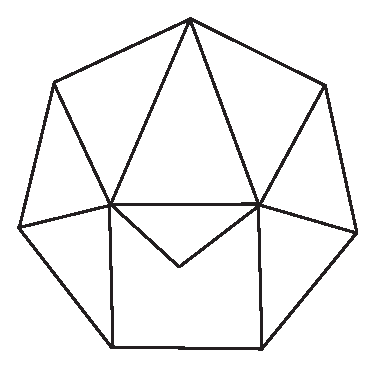
\includegraphics{PS/doubledegree6.eps}
  \caption{Non-adjacent vertices of degree $6$ on a pentagon}
  \label{fig:doubledegree6}
\end{figure}

\begin{proof}
We begin with the first part of the lemma. The sum  $\tau_F(D)$
over these six standard regions is at least
    $$t_5+\tauLP(5,0,2\pi-1.153)> t_8.$$
Similarly,
    $$s_5+\sLP(5,0,2\pi-1.153)<s_8.$$
%
We note that there can be at most one exceptional region with a
vertex of degree six.  Indeed, if there are two, then they must
both be vertices of the same pentagon:
    $$t_8+t_5>\squander.$$
Such a second vertex on the octagonal aggregate leads to one of
the follow constants greater than $\squander$.  These same
constants show that such a second vertex on a hexagonal aggregate
must share two triangular faces with the first vertex of degree
six.
$$\begin{array}{lll}
    t_8 &+\tauLP(4,0,2\pi-1.32-0.8638),\quad\text{or}\\
    t_8 &+1.47\,\pt+\tauLP(4,0,2\pi-1.153-0.8638),\quad\text{or}\\
    t_8 &+\tauLP(5,0,2\pi-1.153) .
\end{array}
$$
(The relevant constants are found at Lemma~\ref{lemma:1.47} and
Lemma~\ref{lemma:0.8638}.)

%We conclude that this case can be fed into the classification
%algorithm as an octagonal face.  We return to this case briefly in
%Section \ref{sec:3.10}, after all relevant plane graphs are
%classified.
\end{proof}

\section{A Non-contravening Four-circuit}
\label{sec:impossible}

This subsection rules out the existence of a particular
four-circuit on a contravening plane graph.  The interior of the
circuit consists of two faces: a triangle and a pentagon.  The
circuit and its enclosed vertex are show in
Figure~\ref{fig:no4circuit:bis} with vertices marked
$p_1,\ldots,p_5$. The vertex $p_1$ is the enclosed vertex, the
triangle is $(p_1,p_2,p_5)$ and the pentagon is
$(p_1,\ldots,p_5)$.  Let $v_1,\ldots,v_4,v_5$ be the corresponding
vertices of $U(D)$.

The diagonals $\{v_5,v_3\}$ and $\{v_2,v_4\}$ have length at least
$2\sqrt2$ by Lemma~\ref{lemma:2t0-doesnt-pass-through}.  If an
interior angle of the  quadrilateral is less than $1.32$, then by
Lemma~\ref{lemma:1.32:bis},  $|v_1-v_3|\le\sqrt{8}$.  Thus, we
assume in the following lemma, that all interior angles of the
quadrilateral aggregate are at least $1.32$.

\begin{lemma}\label{lemma:nobad4}
A decomposition star that contains this configuration does not
contravene.
\end{lemma}

\begin{proof}
Let $P$ denote the quadrilateral aggregate of these two standard
regions. By Lemma~\ref{lemma:11.16:bis}, we have $\tau_P(D)\ge
11.16\,\pt$. There are no other exceptional faces, because
$11.16\,\pt+t_5>\squander$. Every vertex not on $P$ has type
$(5,0)$, by Lemma~\ref{lemma:pq:bis}. In particular, there are no
quadrilateral regions.  The interior angles of $P$ are at least
$1.32$. There are at most $4$ triangles at every vertex of $P$,
because
    $$
    11.16\,\pt+\tauLP(5,0,2\pi-1.32)>\squander.
    $$
    %6.02\,\pt$.
There are at least $3$ triangles at every vertex of $P$, otherwise
we contradict Lemma~\ref{lemma:no-enclosed-tri:bis} or
Lemma~\ref{lemma:no-2}.

The only triangulation with these properties is obtained by
removing one edge from the icosahedron (Exercise).  This implies
that there are two opposite corners of $P$ each having four
quasi-regular tetrahedra. Since the diagonals of $P$ have lengths
greater than $2\sqrt{2}$, the results of \calc{325738864} show
that the union $F$ of these eight quasi-regular tetrahedra
satisfies
    $$
    \tau_F(D) \ge 2(1.5)\,\pt.
    $$
There are two additional vertices of type $(5,0)$ whose tetrahedra
are distinct from these eight quasi-regular tetrahedra. They give
an additional $2(0.55)\,\pt$. Now
$(11.16+2(1.5)+2(0.55))\,\pt>\squander$ by
Lemma~\ref{lemma:0.55:bis}.   The result follows.
\end{proof}


\begin{lemma} \label{lemma:deg5}
A contravening plane graph satisfies Property
\ref{definition:tame:degreeE} of tameness: If a vertex is
contained in an exceptional face, then the degree of the vertex is
at most $5$.
\end{lemma}

\begin{proof} Each vertex of a standard region that bounds $6$
or standard regions, must be one of the vertices of a pentagonal
region by Lemma~\ref{lemma:aggregate6}.  If that pentagonal region
has two or more such vertices, then by the same lemma, it must be
the arrangement shown in Figure~\ref{fig:doubledegree6}.  This
arrangement does not appear on a contravening graph by
Lemma~\ref{lemma:nobad4}.
\end{proof}

\begin{remark}
We have now fully justified the claim made in
Remark~\ref{remark:degree6}: there is at most one vertex on six
standard regions, and it is part of an aggregate in such a way
that it does not appear as the vertex of $G(D)$.
\end{remark}


\section{Possible four-circuits}

Every $4$-circuit divides a plane graph into two aggregates of
faces that we may call the interior and exterior.  We call
vertices of the faces in the aggregate that do not lie on the
$4$-cycle {\it enclosed vertices}.  Thus, every vertex lies in the
$4$-cycle, is enclosed over the interior, or is enclosed over the
exterior.
%
 \index{enclosed vertex}

Lemma~\ref{lemma:no-2} asserts that either the interior or the
exterior has at most $1$ enclosed vertex.   When choosing which
aggregate is to be called the interior, we may make our choice so
that the interior has area at most $2\pi$, and hence contains at
most $1$ vertex. With this choice, we have the following
proposition.

\begin{proposition}
Let $D$ be a contravening plane graph.  A $4$-circuit surrounds one
of the aggregates of faces shown in Property
    \ref{definition:tame:4-circuit} of tameness.
\end{proposition}

\begin{proof}
If there are no enclosed vertices, then the only possibilities are
for it to be a single quadrilateral face or a pair of adjacent
triangles.

Assume there is one enclosed vertex $v$.  If $v$ is connected to
$3$ or $4$ vertices of the quadrilateral, then that possibility is
listed as part of the conclusion.

If $v$ is connected to $2$ opposite vertices in the $4$-cycle,
then the vertex $v$ has type $(0,2)$ and the bounds of
Lemma~\ref{lemma:pq:bis} show that the graph cannot be
contravening.

If $v$ is connected to $2$ adjacent vertices in the $4$-cycle,
then we appeal to Lemma~\ref{lemma:nobad4} to conclude that the
graph does not contravene.

If $v$ is connected to $0$ or $1$ vertices, then we appeal to
Lemma~\ref{lemma:enclosed:bis}.  This completes the proof.
\end{proof}

\chapter{Weight Assignments}
    \label{sec:weight}

The purpose of this section is to prove the existence of a good
admissible weight assignment for contravening plane graphs.  This
will complete the proof that all contravening graphs are tame.

\begin{theorem}  Every contravening plane graph has an admissible
weight assignment of total weight less than $\op{tgt}=14.8$.
\end{theorem}

Given a contravening decomposition star $D$, we define a weight
assignment $w$ by
    $$F \mapsto w(F) = \tau_F(D)/\pt.$$
Since $D$ contravenes,
    $$
    \begin{array}{lll}
    \sum_F w(F) &= \sum_F \tau_F(D)/\pt \\
            &= \tau(D)/\pt\,\le\,\squander/\pt \\
        &< \op{tgt}=14.8.
    \end{array}
    $$
The challenge of the theorem will be to prove that $w$, when
defined by this formula, is admissible.

\section{Admissibility}
\label{sec:admissibility}

The next three lemmas establish that this definition of $w(F)$ for
contravening plane graphs satisfies the first three defining
properties of an admissible weight assignment.

\begin{lemma}  Let $F$ be a face of length $n$ in a contravening plane graph.
Define $w(F)$ as above. Then
        $w(F) \ge d(n)$.
\end{lemma}

\begin{proof} This is Proposition \ref{proposition:wttau}.
\end{proof}

\begin{lemma} Let $v$ be a vertex of type $(p,q)$ in a
contravening plane graph.  Define $w(F)$ as above. Then
        $$\sum_{v\in F} w(F) \ge b(p,q).$$
\end{lemma}


\begin{proof} This is Lemma~\ref{lemma:pq:bis}.
\end{proof}

\begin{lemma} Let $V$ be any set of vertices of type $(5,0)$ in a
contravening plane graph.  Define $w(F)$ as above.
        If the cardinality of $V$ is $k\le 4$,
        then
        $$\sum_{V\cap F\ne\emptyset} w(F) \ge 0.55 k.$$
\end{lemma}

\begin{proof} This is Lemma~\ref{lemma:0.55:bis}.
\end{proof}

The following proposition establishes the final property that
$w(F)$ must satisfy to make it admissible.  {\it Separated sets\/}
are defined in Section~\ref{sec:wtassign}.

\begin{proposition}
        \label{proposition:excess}
        Let $V$ be any separated set \index{separated set}
        of vertices in a contravening plane graph.
        Define $w(F)$ as above.
        Then
        $$\sum_{V\cap F\ne\emptyset} (w(F) -d(len(F)))
            \ge \sum_{v\in V} a(tri(v)),$$
        where $tri(v)$ denotes the number of triangles containing
        the vertex $v$.
\end{proposition}

The proof will occupy the rest of this \chap. Since the degree of
each vertex is five, and there is at least one face that is not a
triangle at the vertex, the only constants $tri(v)$ that arise are
    $$tri(v) \in\{0,\ldots,4\}$$
We will prove that in a contravening plane graph that the
Properties (1) and (4) of a separated set are incompatible with
the condition $tri(v)\le 2$, for some $v\in V$.  This will allows
us to assume that $$tri(v)\in\{3,4\},$$ for all $v\in V$.  These
cases will be treated in Section~\ref{sec:tri34}.


First we prove the inequality when there are no aggregates
involved.  Afterwards, we show that the conclusions can be
extended to aggregate faces as well.

\section{Proof that $tri(v)>2$}
%subsection
\label{sec:2.4} \label{sec:tri2}

In this subsection $D$ is a contravening decomposition star with
associated graph $G(D)$.  Let $V$ be a separated set of vertices
in $G(D)$. Let $v$ be a vertex in $V$ such that none of its faces
is an aggregate in the sense of Remarks \ref{remark:tri-pent} and
\ref{remark:degree6}.

\begin{lemma}  Under these conditions, for every $v\in V$,
$tri(v)>1$.
\end{lemma}

\begin{proof}
If there are $p$ triangles, $q$ quadrilaterals, and $r$ other
faces, then
    $$
    \begin{array}{lll}
    \tau(D) &\ge\sum_{v\in R}\tau_R(D)\\
        &\ge r\, t_5 + \tauLP(p,q,2\pi-r(1.153)).
    \end{array}
    $$ If there is a vertex $w$ that is
not on any of the faces containing $v$, then the sum of
$\tau_F(D)$ over the faces containing $w$ yield an additional
$0.55\,\pt$ by Lemma~\ref{lemma:0.55:bis}. We calculate these
constants for each $(p,q,r)$ and find that the bound is always
greater than $\squander$. This implies that $D$ cannot be
contravening.
$$\begin{array}{llll}
    (p,q,r)&\hbox{\it lower bound }&\hbox{\it justification}\\
    &\\
    (0,5,0)&22.27\,\pt&\text{Lemma~\ref{lemma:pq:bis}}\\
    (0,q,r\ge1)& t_5+4 t_4\approx 14.41\,\pt& \\
    (1,4,0) &17.62\,\pt &\text{Lemma~\ref{lemma:pq:bis}}\\
    (1,3,1) &t_5 + 12.58\,\pt &(\tauLP)\\
    (1,2,2) &2t_5 + 7.53\,\pt &(\tauLP)\\
    (1,q,r\ge3)& 3 t_5 + t_4& \\
\end{array}
$$
\end{proof}


\begin{lemma} Under these same conditions, for every $v\in V$,
$tri(v)>2$.
\end{lemma}

\begin{proof}
Assume that $tri(v)=2$.  We will show that this implies that $D$
does not contravene.  Let $e$ be the number of exceptional faces
at $v$.  We have $e+tri(v)\le5$.

The constants $0.55\,\pt$ and $0.48\,\pt$ used throughout the
proof come from Lemma~\ref{lemma:0.55:bis}. The constants $t_n$
comes from Lemma~\ref{lemma:sn-tn}.

($e=3$): First, assume that there are three exceptional faces
around vertex $v$. They must all be pentagons
($2t_5+t_6>\squander$). The aggregate of the five faces is an
$m$-gon (some $m\le11$).  If there is a vertex not on this
aggregate, use $3t_5+0.55\,\pt>\squander$. So there are at most
nine triangles away from the aggregate, and
    $$
    \sigma(D) \le 9\,\pt + (3 s_5+2\,\pt) < 8\,\pt.
    $$

The argument if there is a quad, pentagon, and hexagon is the same
$(t_4+t_6=2t_5,s_4+s_6=2s_5)$.

($e=2$): Assume next that there are two pentagons and a
quadrilateral around the vertex. The aggregate of the two
pentagons, quadrilateral, and two triangles is an $m$-gon (some
$m\le10$). There must be a vertex not on the aggregate of five
faces, for otherwise we have
    $$
    \sigma(D) \le 8\,\pt+(2s_5+2\,\pt)<8\,\pt.
    $$

The interior angle of one of the pentagons is at most $1.32$.  For
otherwise, $\tauLP(2,1,2\pi-2(1.32))+2t_5+0.55\,\pt>\squander$.

Lemma~\ref{lemma:1.47} shows that any pentagon $R$ with an
interior angle less than $1.32$ yields $\tau_R(D)\ge t_5+
(1.47\,\pt)$. If both pentagons have an interior angle $<1.32$ the
lemma follows easily from this calculation:
    $2(t_5+1.47\,\pt)\,\pt+\tauLP(2,1,2\pi-2(1.153))+0.55\,\pt>\squander$.
If there is one pentagon with angle $>1.32$, we then have
    $t_5+(1.47\,\pt)+\tauLP(2,1,2\pi-1.153-1.32)+t_5+0.55\,\pt>\squander$.


($e=1$): Assume finally that there is one exceptional face at the
vertex. If it is a hexagon (or more), we are done
$t_6+\tauLP(2,2,2\pi-1.153)>\squander$. Assume it is a pentagon. The
aggregate of the five faces at the vertex is bounded by an
$m$-circuit (some $m\le9$). If there are no more than $9$
quasi-regular tetrahedra outside the aggregate, then $\sigma(D)$ is
at most $(9-2(0.48))\,\pt+s_5+\sLP(2,2,2\pi-1.153)<8\,\pt$
(Lemma~\ref{lemma:0.55:bis}). So we may assume that there are at
least three vertices not on the aggregate.

If the interior angle of the pentagon is greater than $1.32$, we
have
$$\tauLP(2,2,2\pi-1.32) +3(0.55)\,\pt +t_5 > \squander;$$
and if it is less than $1.32$, we have by Lemma~\ref{lemma:1.47}
    $$
    \begin{array}{lll}
        \tauLP(2,2,2\pi-1.153)&+3(0.55)\pt+1.47\,\pt+t_5 \\
            &> \squander.
    \end{array}
    $$
\end{proof}

\begin{lemma} The bound $tri(v)>2$ holds if $v$ is a vertex
of an aggregate face.
\end{lemma}

\begin{proof}
The exceptional region enters into the preceding two proofs in a
purely formal way.  Pentagons enter through the bounds
    $$t_5,\ s_5,\ 1.47\,\pt$$
and angles $1.153$, $1.32$.  Hexagons enter through the bounds
    $$t_6,\ s_6$$
and so forth.  These bounds hold for the aggregate faces.  Hence
the proofs hold for aggregates as well.
\end{proof}

\section{Bounds when $tri(v)\in\{3,4\}$.  } %subsection
\label{sec:2.7} \label{sec:tri34}

In this subsection $D$ is a contravening decomposition star with
associated graph $G(D)$.  Let $V$ be a separated set of vertices.
For every vertex  $v$ in $V$, we assume that none of its faces is
an aggregate in the sense of Remarks \ref{remark:tri-pent} and
\ref{remark:degree6}.  We assume that there are three or four
triangles containing $v$, for every $v\in V$.

To prove the Inequality \ref{definition:admissible:excess} in the
definition of admissible weight assignments, we will rely on the
following reductions. Define an equivalence relation on
exceptional faces by $F\sim F'$ if there is a sequence
$F_0=F,\ldots, F_r=F'$ of exceptional faces such that consecutive
faces share a vertex of type $(3,0,2)$. (That is, $tri(v)=3$.)
Let ${\cal F}$ be an equivalence class of faces.

\begin{lemma} Let $V$ be a separated set of vertices.  For every
equivalence class of exceptional faces $\cal F$, let $V({\cal F})$
be the subset of $V$ whose vertices lie in the union of faces of
${\cal F}$. Suppose that for every equivalence class $\cal F$, the
Inequality \ref{definition:admissible:excess} (in the definition
of admissible weight assignments) holds for $V({\cal F})$. Then
the Inequality holds for $V$.
\end{lemma}

\begin{proof}
By construction, each vertex in $V$ lies in some $F$, for an
exceptional face.  Moreover, the separating property of $V$
insures that the triangles and quadrilaterals in the inequality
are associated with a well-defined  ${\cal F}$. Thus, the
inequality for $V$ is a sum of the inequalities for each $V({\cal
F})$.
\end{proof}


\begin{lemma}
\label{lemma:split}
 Let $v$ be a vertex in a separated set $V$ at which there are $p$
triangles, $q$ quadrilaterals, and $r$ other faces.  Suppose that
for some $p'\le p$ and $q'\le q$, we have
    $$\tauLP(p',q',\alpha) > ( p' d(3) + q' d(4) + a(p))\,\pt$$
for some upper bound $\alpha$ on the angle occupied by $p'$
triangles and $q'$ quadrilaterals at $v$.  Suppose further that
the Inequality \ref{definition:admissible:excess} (in the
definition of admissible weight assignments) holds for the
separated set $V' = V\setminus \{v\}$. Then the inequality holds
for $V$.
\end{lemma}

\begin{proof}  Let $F_1,\ldots,F_m$, $m={p'+q'}$, be faces corresponding
to the triangles and quadrilaterals in the lemma.  The hypotheses
of the lemma imply that
    $$\sum_{1}^{m} (w{F_i}(D) - d(len(F_i))) > a(p).$$
Clearly, the Inequality for $V$ is the sum of this inequality, the
inequality for $V'$, and $d(n)\ge0$.
\end{proof}


Recall that the central vertex of a flat quarter is defined to be
the one that does not lie on the triangle formed by the origin and
the diagonal.
%
 \index{central}

\begin{lemma} \label{lemma:excess-1:bis}
Let $R$ be an exceptional standard region.  Let $V$
be a set of vertices of $R$.  If $v\in V$, let $p_v$ be the number
of triangular regions at $v$ and let $q_v$ be the number of
quadrilateral regions at $v$.  Assume that $V$ has the following
properties:
    \begin{enumerate}
        \item The set $V$ is separated.
        \item If $v\in V$, then there are five standard regions at
        $v$.
        \item If $v\in V$, then the corner over $v$ is a central
        vertex of a flat quarter in the cone over $R$.
        \item If $v\in V$, then $p_v\ge 3$.  That is, at least
        three of the five standard regions at $v$ are triangular.
        \item If $R'\ne R$ is an exceptional region at $v$, and if $R$
        has interior angle at least $1.32$ at $v$, then $R'$ also has interior
        angle at least $1.32$ at $v$.
    \end{enumerate}
Let $F$ be the union of $\{R\}$ with the set of triangular and
quadrilateral regions that have a vertex at some $v\in V$. Then
    $$\tau_F(D) > \sum_{v\in V} (p_v d(3) + q_v d(4) + a
    (p_v))\,\pt.$$
\end{lemma}

\begin{proof} If $(p_v,q_v)=(3,1)$ and the internal angle of $R$ at $v$ is at
least $1.32$, then we use
   $$\tauLP(3,1,2\pi-1.32) > 1.4\,\pt + t_4.$$
In this case, the inequality of the Lemma is a consequence of this
inequality and the inequality for $V\setminus\{v\}$.  Thus, we may
assume without loss of generality that if $(p_v,q_v)=(3,1)$, then
the internal angle of $R$ at $v$ is at most $1.32$.
  \shortversion{The conclusion is now found
in \cite{KC}.}
    \longversion{The conclusion now follows from Lemma~\ref{lemma:excess-1}.}
\end{proof}

\begin{lemma}  Property \ref{definition:admissible:excess}  of
admissibility holds.  That is, let $V$ be any separated set of
vertices. Then
        $$\sum_{F:\,V\cap F\ne\emptyset} (w(F) -d(len(F)))
            \ge \sum_{v\in V} a(tri(v)).$$
\end{lemma}

\begin{proof}  Let $V$ be a separated set of vertices.
The results of Section~\ref{sec:tri2} reduce the lemma to the case
where $tri(v)\in\{3,4\}$ for every vertex $v\in V$.

We will say that there is a flat quarter centered at $v$, if the
corner $v'$ over $v$ is the central vertex of a flat quarter and
that flat quarter lies in the cone over an exceptional region.

One case is easy to deal with.  Assume that there are three
triangles, a quadrilateral, and an exceptional face at the vertex.
Assume the interior angle on the exceptional region is least
$1.32$, then
    \begin{equation}
    \tauLP(3,1,2\pi-1.32)>1.4\,\pt + t_4.
    \label{eqn:tau1.32}
    \end{equation}
This gives the bound in the sense of Lemma~\ref{lemma:split} at
such a vertex. For the rest of the proof, assume that the interior
angle on the exceptional region is less than $1.32$ at vertices of
type $(p,q,r)=(3,1,1)$. This implies in particular by
Lemma~\ref{lemma:1.32:bis} that there is a flat quarter centered
at each vertex of this type.

Let $v$ be vertex with no flat quarter centered at $v$.   By
Lemma~\ref{lemma:1.32:bis}, the interior angles of the
exceptional regions at $v$ are at least $1.32$.   It follows%
\footnote{\calc{551665569}, \calc{824762926}, and
\calc{325738864}}
%% K.C.-2002-version: 17.20 Group 20, 17.21 Group 21. (page 49).
that
    \begin{equation}
    \tauLP(p_v,q_v,\alpha) > ( p_v d(3) + q_v d(4) + a(p_v))\,\pt.
    \label{eqn:tau-alpha}
    \end{equation}
Thus, by Lemma~\ref{lemma:split}, we reduce to the case where for
each $v\in V$,  there is flat quarter centered at $v$. Assume that
$V$ has this property.

Pick a function $f$ from the set $V$ to the set of exceptional
standard regions as follows. If there is only one exceptional
region at $v$, then let $f(v)$ be that exceptional region. If
there are two exception regions at $v$, then let $f(v)$ be one of
these two exceptional regions.  Pick it to be an exceptional
region with interior angle at most $1.32$ if one of the two
exceptional regions has this property. Pick it to have a flat
quarter centered at $v$. Note that by Lemma~\ref{lemma:1.32:bis},
if the exceptional region has interior angle at most $1.32$, then
$f(v)$ will have a flat quarter centered at $v$.

For each exceptional region $R$, let
    $$V_R = \{ v\in V : f(v) = R\}.$$
By Lemma~\ref{lemma:excess-1:bis}, the Property
\ref{definition:admissible:excess} of admissibility is satisfied
for each $V_R$.  Since this property is additive in $V_R$ and
since $V$ is the disjoint union of the sets $V_R$, the proof is
complete.
\end{proof}


%\chapter{The Aggregate Cases}
%    \label{sec:aggregate}

\section{Weight Assignments for Aggregates}

\begin{lemma}
Consider a separated set of vertices $V$ on an aggregated face $F$
as in Remark \ref{remark:tri-pent}.  Then Inequality
\ref{definition:admissible:excess} holds (in the definition of
admissible weight assignments):
    $$\sum_{V\cap F\ne\emptyset} (w(F) -d(len(F)))
            \ge \sum_{v\in V} a(tri(v)).$$
\end{lemma}

\begin{proof}
We may assume that $tri(v)\in\{3,4\}$.

First consider the aggregate of Remark \ref{remark:tri-pent} of a
triangle and eight-sided region, with pentagonal hull $F$. There
is no other exceptional region in a contravening decomposition
star with this aggregate:
    $$t_8 + t_5 > \squander.$$
A separated set of vertices $V$ on $F$ has cardinality at most
$2$.  This gives the desired bound $$t_8 > t_5 + 2 (1.5)\,\pt.$$

Next, consider the aggregate of a hexagonal hull with an enclosed
vertex.  Again, there is no other exceptional face. If there are
at most $k\le 2$ vertices in a separated set, then the result
follows from
    $$t_8 > t_6 + k (1.5)\,\pt.$$
There are at most three vertices in $V$ on a hexagon, by the
non-adjacency conditions defining $V$. A vertex $v$ can be removed
from $V$ if it is not the central vertex of a flat quarter (Lemma
\ref{lemma:split} and Inequalities~\ref{eqn:tau1.32} and
\ref{eqn:tau-alpha}). If there is an enclosed vertex $w$, it is
impossible for there to be three nonadjacent vertices, each the
central vertex of a flat quarter:
    $$\CalE(2,2,2,\sqrt8,\sqrt8,\sqrt8,2t_0,2t_0,2)>2t_0.$$
($\CalE$ is defined in Definition~\ref{def:calE}.)

Finally consider the aggregate of a pentagonal hull with an
enclosed vertex.  There are at most $k\le2$ vertices in a
separated set in $F$.  There is no other exceptional region:
    $$t_7 + t_5 > \squander.$$
The result follows from
    $$t_7 > t_5 + 2(1.5)\,\pt.$$
\end{proof}

\begin{lemma}
Consider a separated set of vertices $V$ on an aggregate face of a
contravening plane graph as in Remark~\ref{remark:degree6}.  The
Inequality~\ref{definition:admissible:excess} holds in the
definition of admissible weight assignments.
\end{lemma}

\begin{proof}
There is at most one exceptional face in the plane graph:
    $$t_8 + t_5 > \squander.$$
Assume first that aggregate face is an octagon (Figure
\ref{fig:degree6}). At each of the vertices of the face that lies
on a triangular standard region in the aggregate, we can remove
the vertex from $V$ using Lemma \ref {lemma:split} and the
estimate
    $$\tauLP(4,0,2\pi-2 (0.8638)) > 1.5\,\pt.$$
This leaves at most one vertex in $V$, and it lies on a vertex of
$F$ which is ``not aggregated,'' so that there are five standard
regions of the associated decomposition star at that vertex, and
one of those regions is pentagonal.  The value $a(4)=1.5\,\pt$ can
be estimated at this vertex in the same way it is done for a
non-aggregated case in Section~\ref{sec:tri34}.

Now consider the case of an aggregate face that is a hexagon
(Figure \ref{fig:degree6}).  The argument is the same: we reduce
to $V$ containing a single vertex, and argue that this vertex can
be treated as in Section~\ref{sec:tri34}.  (Alternatively, use the
fact that the pentagon-triangle combination in this aggregate has
been eliminated by Lemma~\ref{lemma:nobad4}.)
\end{proof}


%It has now been verified that all the properties of tameness
%except one have been verified.  This section verifies that
%contravening plane graphs satisfy this final property, and in this
%way we complete the proof that all contravening plane graphs are
%tame.




The proof that contravening plane graphs are tame is complete.
